%%%%%%%%%%%%%%%%%%%%%%%%%%%%%%%%%%%%%%%%%%%%%%%%%%%%%%%%%%%%%%%%%%%%%%%%%%%%%%%%%%%%%%%%%%%%%%%%%%%%%%%
%%%%%%%%%%%%%% Template de Artigo Adaptado para Trabalho de Diplomação do ICEI %%%%%%%%%%%%%%%%%%%%%%%%
%% codificação UTF-8 - Abntex - Latex -  							     %%
%% Autor:    Fábio Leandro Rodrigues Cordeiro  (fabioleandro@pucminas.br)                            %% 
%% Co-autores: Prof. João Paulo Domingos Silva, Harison da Silva e Anderson Carvalho		     %%
%% Revisores normas NBR (Padrão PUC Minas): Helenice Rego Cunha e Prof. Theldo Cruz                  %%
%% Versão: 1.1     18 de dezembro 2015                                                               %%
%%%%%%%%%%%%%%%%%%%%%%%%%%%%%%%%%%%%%%%%%%%%%%%%%%%%%%%%%%%%%%%%%%%%%%%%%%%%%%%%%%%%%%%%%%%%%%%%%%%%%%%
\section{\esp Dispositivos Lógicos Programáveis}

São diversas as tecnologias utilizadas nas construções de circuitos porém os termos que aqui tratados foram antecipadamente especificados e atenderão fielmente ao enunciado proposto.


\subsection{\esp ASICs}

São caratecterizados especialmente por requerir de um processo especial de fabricação, dando a este um alto custo de projeto e longa implementação, quando utilizado em grandes projetos, procura-se fazer uma divisão de testes para tentar melhorar o desempenho.

\subsection{\esp ASSP}

Não foi encontrado o conceito.

\subsection{\esp SPLD}

É um circuto que menos tem custo e possui um desempenho diante os outros. Composto principalmente por portas AND/OR (simples) e pode ter ou não flip-flops na saída.

\subsection{\esp CPLD}

CPLDs são dispositivos programáveis e reprográmaveis pelo usuário, com alto desempenho, baixo custo e alta capacidade de integração.

\subsection{\esp SOC}
Não foi encontrado o conceito.

\subsection{\esp FPGA}

Os FPGAs não possuem planos de port OR/AND, usam na verdade grande arranjo de célula configurável que são implementadas em funções lógicas. Tem como principais recursos: blocos lógicos, blocos de entrada e saída e chaves de interconexão.






\section{\esp Diferenciar}

\subsection{\esp PROM}

São memórias de apenas leitura, porém após a evolução das máquinas, esta permite a programação de usuários.

% Tabela
\begin{table}[htb]
	\centering
	\caption{\hspace{0.1cm} Tabela verdade do decodificador (PROM 8X2)}
	\vspace{-0.3cm} % espaço entre titulo e tabela
	\label{tab:tabela1}
	% Conteúdo da tabela
	\begin{tabular}{l|c |c | c | c}
  \hline
    \textbf{X}	& \textbf{Y} & \textbf{Z}  & \textbf{EXIT 1} & \textbf{EXIT 2} \\
    \hline
        0	& 0 & 0 &  0  &  1  \\
        1	& 0 &  0 & 1 & 1  \\
        0	& 1 & 0 & 1 & 0  \\
        1   &  1 & 0 & 0 & 0  \\
        0	& 0  &  1 & 0 & 1 \\
        1   &  0 & 1 & 0 & 1  \\
        0  & 1  &  1 & 1 & 0 \\
        1  & 1  &  1 & 1 & 1 \\
     \hline
 \end{tabular}
 	\vspace{.1cm}  %espaço entre tabela e fonte
	\small
	% Fonte
	{\footnotesize\\ \textbf{Fonte: “DISPOSITIVOS LÓGICOS PROGRAMÁVEIS”. Profa. Luiza Maria Romeiro Codá. Departamento de Engenharia Elétrica e de Computação.  Acessado em 27/03/2022}}
\end{table}



\subsection{\esp PLA}

Um PLA \textit{(Programmable Logic Array)} um conjunto de arranjos de AND e OR, onde ambos são programáveis e por isso possui um desempenho bom em somo da produtos pois possuem muitas portas.

 \ref{fig:figura1}. 
% Figura
\begin{figure}[ht]
	\centering	
	\caption[\hspace{0.1cm}]{PLA de quatro entradas programadas}
  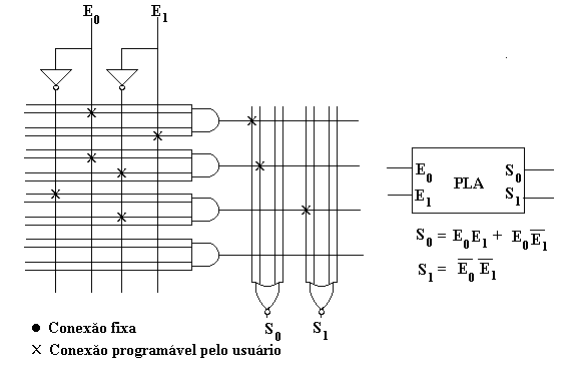
\includegraphics[width=0.4\textwidth]{figuras/pla.png}
	% Caption centralizada
% 	\captionsetup{justification=centering}
	% Caption e fonte 
	 \vspace{-0.2cm}
	\\\textbf{\footnotesize Fonte: Profa. Luiza Maria Romeiro Codá "DISPOSITIVOS LÓGICOS PROGRAMÁVEIS”}
	\label{fig:figura1}
\end{figure}
\vspace{-0.5cm}


\subsection{\esp PAL}

Corresponde a uma matriz lógica programável, é uma forma simplificada da PLA, sendo apenas as portas AND programavél, a matriz OR é fixa.

 \ref{fig:figura1}. 
% Figura
\begin{figure}[ht]
	\centering	
	\caption[\hspace{0.1cm}]{PAL de quatro entradas programadas}
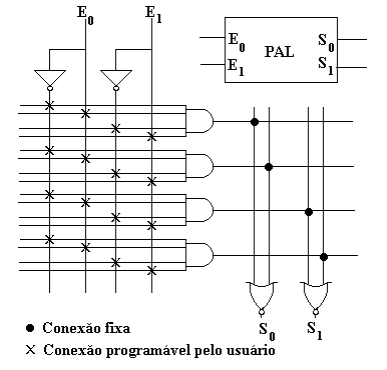
\includegraphics[width=0.4\textwidth]{figuras/PAL.png}
	% Caption centralizada
% 	\captionsetup{justification=centering}
	% Caption e fonte 
	 \vspace{-0.2cm}
	\\\textbf{\footnotesize Fonte: Profa. Luiza Maria Romeiro Codá "DISPOSITIVOS LÓGICOS PROGRAMÁVEIS”}
	\label{fig:figura1}
\end{figure}
\vspace{-0.5cm}


\section{\esp Comparação e diferenciação}

\subsection{\esp CPLD}

São caratecterizados especialmente por requerir de um processo especial de fabricação, dando a este um alto custo de projeto e longa implementação, quando utilizado em grandes projetos, procura-se fazer uma divisão de testes para tentar melhorar o desempenho.

 \ref{fig:figura1}. 
% Figura
\begin{figure}[ht]
	\centering	
	\caption[\hspace{0.1cm}]{Estrutura interna do MAX 7000TM}
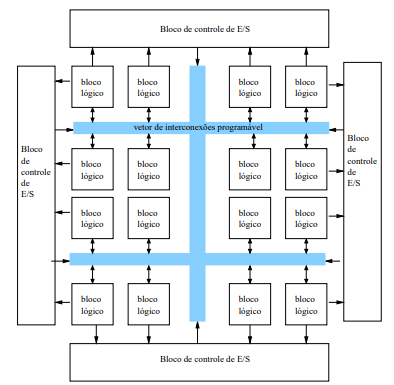
\includegraphics[width=0.4\textwidth]{figuras/CPLD.png}
	% Caption centralizada
% 	\captionsetup{justification=centering}
	% Caption e fonte 
	 \vspace{-0.2cm}
	\\\textbf{\footnotesize Fonte: Relatório Técnico no.005 de 2002, da
área de informática do DCCE \citeonline{cap-livro} }
	\label{fig:figura1}
\end{figure}
\vspace{-0.5cm}

 \newpage \subsection{\esp FPGA}

São caratecterizados especialmente por requerir de um processo especial de fabricação, dando a este um alto custo de projeto e longa implementação, quando utilizado em grandes projetos, procura-se fazer uma divisão de testes para tentar melhorar o desempenho.

 \ref{fig:figura1}. 
% Figura
\begin{figure}[ht]
	\centering	
	\caption[\hspace{0.1cm}]{Configuração interna de uma FPGA}
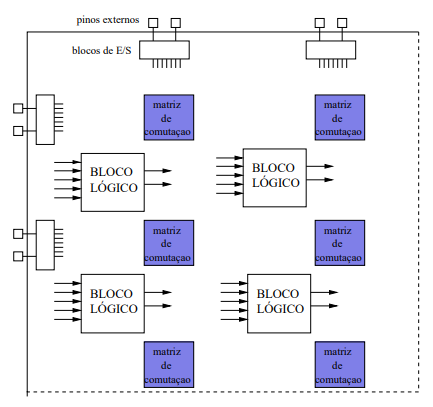
\includegraphics[width=0.4\textwidth]{figuras/FPGA.png}
	% Caption centralizada
% 	\captionsetup{justification=centering}
	% Caption e fonte 
	 \vspace{-0.2cm}
	\\\textbf{\footnotesize Fonte: Relatório Técnico no.005 de 2002, da área de informática do DCCE}
	\label{fig:figura1}
\end{figure}
\vspace{-0.5cm}

\newpage
\section{REFERÊNCIAS}
O.A.C.Macedo; P.B.Alves;  N.Marranghello. DISPOSITIVOS LÓGICOS PROGRAMÁVEIS. UNIVERSIDADE ESTADUAL PAULISTA, nov. 2002.

FREITAS, Tiago Tobias; PASQUALIANOTO, Thiago Luiz; LEÃO, Juliano Carlos Leão.1O CPLD (Dispositivo Complexo de Lógica Programação aplicado em automação industrial. Feira SENAI Paulista de Inovação Tecnológica  -  INOVASENAI, 2005.

 CODÁ, Luiza Maria Romeiro. DISPOSITIVOS LÓGICOS PROGRAMÁVEIS. Departamento de Engenharia Elétrica e de Computação.
 

 
